\section{Evaluation}
\label{sec:evaluation}

We have implemented metadata persistence on the latest version of
DM-Cache running on Linux kernel version 3.3. To evaluate this we use
the workloads offered by the IOZone benchmark to evaluate the overhead
of this mechanism.

For testing we connected two machines via iSCSI. One machine serves as
the iSCSI-target/network-storage and is running Ubuntu 11.10. The
second machine serves as the iSCSI-client running Arch Linux with the
3.3 kernel and issues the storage requests to the iSCSI-target. The
average network latency between the two machines was between 0.3ms and
0.4ms.

We evaluated our approach on an Mtron Pro 7500 64GB SSD. We used an
Mtron SSD to get a good upper bound on our performance overhead as
Mtron SSD's (as compared to Intel and Vertex SSD's) have slower write
performance \cite{FIOS}.

To evaluate the improvement of batching we simply keep track of all
metadata writes and we keep a counter that keeps track of the number
of times we batch a metadata write with a pending update on that same
metadata block.

Due to issues with the implementation of the write-back mechanism
within DM-Cache we only show evaluation of DM-Cache using our
persistence mechanism with write-through. Our testing shows no issues
with the actual data when running experiments but the kernel logs show
some file-system warnings so we omit those results.

\subsection{IOZone}

We use the IOZone benchmark to evaluate the throughput of DM-Cache as
a cold cache with and without metadata persistence enabled as well as
a warm cache with and without metadata persistence enabled to
calculate the overhead.

Because we are only using the write-through mechanism in our
evaluation the only throughput results that are meaningful to us are
the read throughput statistics. Reread is not significant because that
will use the data that is cached in RAM.

For each test run we create and initialize a new cache and run IOZone
on different sized caches and record the results. We use cache sizes
of 512MB, 1GB and 2GB. To evaluate the results of a warm cache we
simply run the read workload in IOZone and then drop the page cache
for the system so that it is forced to do I/O rather than simply
reading the information from RAM while the information is still stored
in the cache.

\graphicspath{{../Results/}}

\begin{figure}[t]
  \caption{IOZone Read Workload with Cold Cache}
  \centering 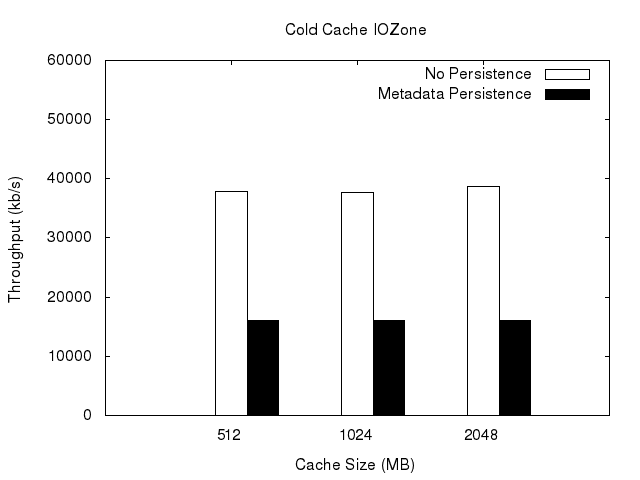
\includegraphics[width=0.5\textwidth]{results_first.png}
  \label{fig:iozone-cold}
\end{figure}

\begin{figure}[t]
  \caption{IOZone Read Workload with Warm Cache}
  \centering 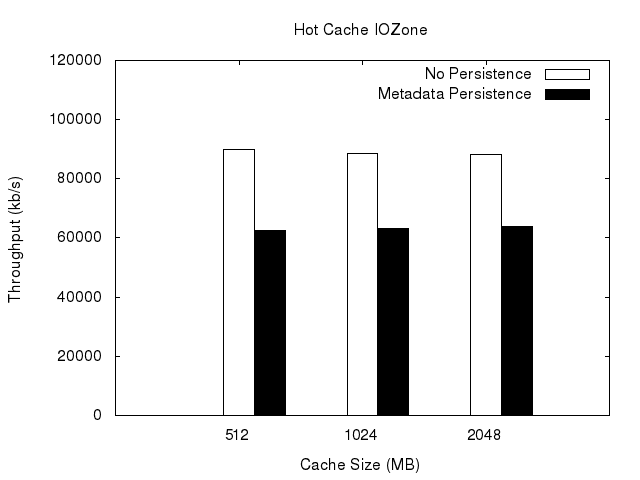
\includegraphics[width=0.5\textwidth]{results_second.png}
  \label{fig:iozone-warm}
\end{figure}

\begin{figure}[t]
  \caption{IOZone Write Workload}
  \centering 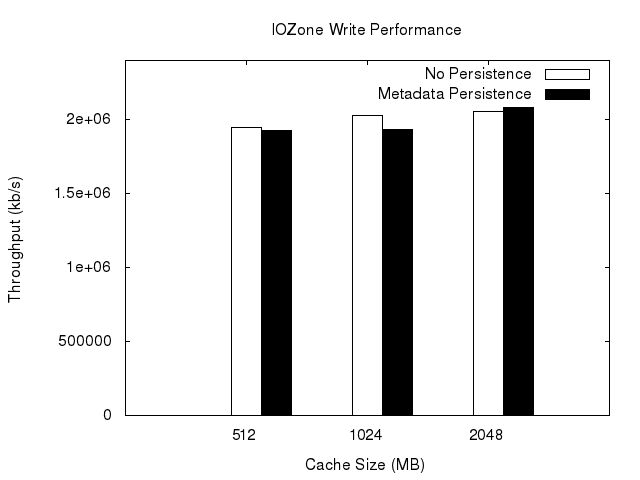
\includegraphics[width=0.5\textwidth]{results_write.png}
  \label{fig:iozone-write}
\end{figure}

In Figure \ref{fig:iozone-cold} it can be seen that inserting a lot of
blocks into the cache along with our metadata persistence mechanism
causing extra writes can slow down performance by about 50\%. This is
because metadata is being updated constantly because every block
fetched is not cached so it has to be written to the cache device
along with relevant metadata for each block. Figure
\ref{fig:iozone-warm} shows that once the cache has reached a state
where access is mostly read hits performance comes closer to a cache
without persistence by about 75\%. The majority of the performance hit
comes from the use of synchronous I/O to ensure that metadata is
written correctly to the disk and that it is always consistent with
the data that is cached on the device. The rest of the performance
loss is due to the slow write efficiency of SSD's in general but in
this case it's also due to the SSD itself. Mtron SSD's are known to
have some of the slowest write times compared to other SSD's
\cite{FIOS}.

To evaluate the computational overhead of the extra code added to
DM-Cache we ran the IOZone write workload on a write-through
cache. The results are shown in Figure~\ref{fig:iozone-write}. These
numbers are the average over three runs of IOZone with the cache being
destroyed and recreated after every run to ensure that no cached data
is being held in memory. The additional code added to DM-Cache does
not seem to affect performance when it comes to additional thinktime
by DM-Cache.

\subsection{Metadata Batching Efficiency}

To evaluate how effective our metadata batching technique we keep two
counters, one for the total number of metadata write operations that
would have happened without batching and another for the amount of
operations that were able to be successfully merged into one batch.

In Table~\ref{table:batching} we can see that a good percentage of the
metadata writes can be batched together to improve the metadata update
performance when many blocks are being updated at once. This gives us
87-88\% less writes overall as we can simply issue one write that
handles many metadata updates at once.

\begin{table}[t]
  \caption{Metadata Batching Statistics for IOZone Read Workload}
  \centering
  \resizebox{0.5\textwidth}{!} {
    \begin{tabular}{ | l | l | l | }
      \hline
      Cache Size (MB) & Metadata Updates & Batched Metadata Updates \\ \hline
      512 & 286,900 & 250,958 \\ \hline
      1024 & 569,317 & 501,770 \\ \hline
      2048 & 860,075 & 752,423 \\
      \hline
    \end{tabular}
  }
  \label{table:batching}
\end{table}
